%%
%% Automatically generated file from DocOnce source
%% (https://github.com/hplgit/doconce/)
%%
%%
% #ifdef PTEX2TEX_EXPLANATION
%%
%% The file follows the ptex2tex extended LaTeX format, see
%% ptex2tex: http://code.google.com/p/ptex2tex/
%%
%% Run
%%      ptex2tex myfile
%% or
%%      doconce ptex2tex myfile
%%
%% to turn myfile.p.tex into an ordinary LaTeX file myfile.tex.
%% (The ptex2tex program: http://code.google.com/p/ptex2tex)
%% Many preprocess options can be added to ptex2tex or doconce ptex2tex
%%
%%      ptex2tex -DMINTED myfile
%%      doconce ptex2tex myfile envir=minted
%%
%% ptex2tex will typeset code environments according to a global or local
%% .ptex2tex.cfg configure file. doconce ptex2tex will typeset code
%% according to options on the command line (just type doconce ptex2tex to
%% see examples). If doconce ptex2tex has envir=minted, it enables the
%% minted style without needing -DMINTED.
% #endif

% #define PREAMBLE

% #ifdef PREAMBLE
%-------------------- begin preamble ----------------------

\documentclass[%
oneside,                 % oneside: electronic viewing, twoside: printing
final,                   % draft: marks overfull hboxes, figures with paths
10pt]{article}

\listfiles               %  print all files needed to compile this document

\usepackage{relsize,makeidx,color,setspace,amsmath,amsfonts,amssymb}
\usepackage[table]{xcolor}
\usepackage{bm,ltablex,microtype}

\usepackage[pdftex]{graphicx}

\usepackage{ptex2tex}
% #ifdef MINTED
\usepackage{minted}
\usemintedstyle{default}
% #endif
\usepackage{fancyvrb}

\usepackage[T1]{fontenc}
%\usepackage[latin1]{inputenc}
\usepackage{ucs}
\usepackage[utf8x]{inputenc}

\usepackage{lmodern}         % Latin Modern fonts derived from Computer Modern

% Hyperlinks in PDF:
\definecolor{linkcolor}{rgb}{0,0,0.4}
\usepackage{hyperref}
\hypersetup{
    breaklinks=true,
    colorlinks=true,
    linkcolor=linkcolor,
    urlcolor=linkcolor,
    citecolor=black,
    filecolor=black,
    %filecolor=blue,
    pdfmenubar=true,
    pdftoolbar=true,
    bookmarksdepth=3   % Uncomment (and tweak) for PDF bookmarks with more levels than the TOC
    }
%\hyperbaseurl{}   % hyperlinks are relative to this root

\setcounter{tocdepth}{2}  % levels in table of contents

% Tricks for having figures close to where they are defined:
% 1. define less restrictive rules for where to put figures
\setcounter{topnumber}{2}
\setcounter{bottomnumber}{2}
\setcounter{totalnumber}{4}
\renewcommand{\topfraction}{0.95}
\renewcommand{\bottomfraction}{0.95}
\renewcommand{\textfraction}{0}
\renewcommand{\floatpagefraction}{0.75}
% floatpagefraction must always be less than topfraction!
% 2. ensure all figures are flushed before next section
\usepackage[section]{placeins}
% 3. enable begin{figure}[H] (often leads to ugly pagebreaks)
%\usepackage{float}\restylefloat{figure}

% --- fancyhdr package for fancy headers ---
\usepackage{fancyhdr}
\fancyhf{} % sets both header and footer to nothing
\renewcommand{\headrulewidth}{0pt}
\fancyfoot[LE,RO]{\thepage}
% Ensure copyright on titlepage (article style) and chapter pages (book style)
\fancypagestyle{plain}{
  \fancyhf{}
  \fancyfoot[C]{{\footnotesize \copyright\ 2023, UP Mathématiques. ESPRIT}}
%  \renewcommand{\footrulewidth}{0mm}
  \renewcommand{\headrulewidth}{0mm}
}
% Ensure copyright on titlepages with \thispagestyle{empty}
\fancypagestyle{empty}{
  \fancyhf{}
  \fancyfoot[C]{{\footnotesize \copyright\ 2023, UP Mathématiques. ESPRIT}}
  \renewcommand{\footrulewidth}{0mm}
  \renewcommand{\headrulewidth}{0mm}
}

\pagestyle{fancy}


\usepackage[framemethod=TikZ]{mdframed}

% --- begin definitions of admonition environments ---

% Admonition style "mdfbox" is an oval colored box based on mdframed
% "notice" admon
\colorlet{mdfbox_notice_background}{gray!5}
\newmdenv[
  skipabove=15pt,
  skipbelow=15pt,
  outerlinewidth=0,
  backgroundcolor=mdfbox_notice_background,
  linecolor=black,
  linewidth=2pt,       % frame thickness
  frametitlebackgroundcolor=mdfbox_notice_background,
  frametitlerule=true,
  frametitlefont=\normalfont\bfseries,
  shadow=false,        % frame shadow?
  shadowsize=11pt,
  leftmargin=0,
  rightmargin=0,
  roundcorner=5,
  needspace=0pt,
]{notice_mdfboxmdframed}

\newenvironment{notice_mdfboxadmon}[1][]{
\begin{notice_mdfboxmdframed}[frametitle=#1]
}
{
\end{notice_mdfboxmdframed}
}

% Admonition style "mdfbox" is an oval colored box based on mdframed
% "summary" admon
\colorlet{mdfbox_summary_background}{gray!5}
\newmdenv[
  skipabove=15pt,
  skipbelow=15pt,
  outerlinewidth=0,
  backgroundcolor=mdfbox_summary_background,
  linecolor=black,
  linewidth=2pt,       % frame thickness
  frametitlebackgroundcolor=mdfbox_summary_background,
  frametitlerule=true,
  frametitlefont=\normalfont\bfseries,
  shadow=false,        % frame shadow?
  shadowsize=11pt,
  leftmargin=0,
  rightmargin=0,
  roundcorner=5,
  needspace=0pt,
]{summary_mdfboxmdframed}

\newenvironment{summary_mdfboxadmon}[1][]{
\begin{summary_mdfboxmdframed}[frametitle=#1]
}
{
\end{summary_mdfboxmdframed}
}

% Admonition style "mdfbox" is an oval colored box based on mdframed
% "warning" admon
\colorlet{mdfbox_warning_background}{gray!5}
\newmdenv[
  skipabove=15pt,
  skipbelow=15pt,
  outerlinewidth=0,
  backgroundcolor=mdfbox_warning_background,
  linecolor=black,
  linewidth=2pt,       % frame thickness
  frametitlebackgroundcolor=mdfbox_warning_background,
  frametitlerule=true,
  frametitlefont=\normalfont\bfseries,
  shadow=false,        % frame shadow?
  shadowsize=11pt,
  leftmargin=0,
  rightmargin=0,
  roundcorner=5,
  needspace=0pt,
]{warning_mdfboxmdframed}

\newenvironment{warning_mdfboxadmon}[1][]{
\begin{warning_mdfboxmdframed}[frametitle=#1]
}
{
\end{warning_mdfboxmdframed}
}

% Admonition style "mdfbox" is an oval colored box based on mdframed
% "question" admon
\colorlet{mdfbox_question_background}{gray!5}
\newmdenv[
  skipabove=15pt,
  skipbelow=15pt,
  outerlinewidth=0,
  backgroundcolor=mdfbox_question_background,
  linecolor=black,
  linewidth=2pt,       % frame thickness
  frametitlebackgroundcolor=mdfbox_question_background,
  frametitlerule=true,
  frametitlefont=\normalfont\bfseries,
  shadow=false,        % frame shadow?
  shadowsize=11pt,
  leftmargin=0,
  rightmargin=0,
  roundcorner=5,
  needspace=0pt,
]{question_mdfboxmdframed}

\newenvironment{question_mdfboxadmon}[1][]{
\begin{question_mdfboxmdframed}[frametitle=#1]
}
{
\end{question_mdfboxmdframed}
}

% Admonition style "mdfbox" is an oval colored box based on mdframed
% "block" admon
\colorlet{mdfbox_block_background}{gray!5}
\newmdenv[
  skipabove=15pt,
  skipbelow=15pt,
  outerlinewidth=0,
  backgroundcolor=mdfbox_block_background,
  linecolor=black,
  linewidth=2pt,       % frame thickness
  frametitlebackgroundcolor=mdfbox_block_background,
  frametitlerule=true,
  frametitlefont=\normalfont\bfseries,
  shadow=false,        % frame shadow?
  shadowsize=11pt,
  leftmargin=0,
  rightmargin=0,
  roundcorner=5,
  needspace=0pt,
]{block_mdfboxmdframed}

\newenvironment{block_mdfboxadmon}[1][]{
\begin{block_mdfboxmdframed}[frametitle=#1]
}
{
\end{block_mdfboxmdframed}
}

% --- end of definitions of admonition environments ---

% prevent orhpans and widows
\clubpenalty = 10000
\widowpenalty = 10000

% --- end of standard preamble for documents ---


% insert custom LaTeX commands...

\raggedbottom
\makeindex

%-------------------- end preamble ----------------------

\begin{document}

% matching end for #ifdef PREAMBLE
% #endif

\newcommand{\exercisesection}[1]{\subsection*{#1}}


% ------------------- main content ----------------------



% ----------------- title -------------------------

\title{Introduction à Python}

% ----------------- author(s) -------------------------

\author{UP Mathématiques\inst{1}}
\institute{École Supérieure PRivée d'Ingénierie et de Technologies (ESPRIT).\inst{1}}
% ----------------- end author(s) -------------------------

\date{2 novembre 2023
% <optional titlepage figure>
% <optional copyright>
}

\vspace{6mm}

% inline figure
\centerline{
\includegraphics[width=0.45\linewidth]{imgs/Signature-01.jpg}}

\vspace{6mm}







% !split
\section{Objectifs généraux en premier}

Une partie essentielle de ce cours est de vous permettre de faire de la science par des expériences numériques et de développer des projets qui vous permettent d'étudier des systèmes complexes. Le but est d'améliorer ce que nous appelons la pensée algorithmique.

\paragraph{Algorithme}
Un ensemble fini d'instructions non ambiguës qui, étant donné un ensemble de conditions initiales, peuvent être effectuées dans une séquence prescrite pour atteindre un certain but.

% !split
\section{Situation standard que nous rencontrons quotidiennement}

La situation standard que nous rencontrons presque tous les séances de cours:

\begin{itemize}
\item Théorie + expérience + simulation est presque la norme dans la recherche et l'industrie.

\item Être capable de modéliser des systèmes complexes. Résoudre de vrais problèmes.

\item Accent la compréhension des principes fondamentaux et des lois dans les sciences.

\item Être capable de visualiser, présenter, discuter, interpréter et venir avec une analyse critique des résultats, et développer une attitude éthique saine pour son propre travail.

\item Améliorer le raisonnement sur la méthode scientifique.
\end{itemize}

\noindent
Une bonne présentation des résultats obtenus via de bons rapports scientifiques, aide à inclure tous les aspects ci-dessus.

% !split
\section{Langage Python}

\href{{http://www.python.org/}}{Python} est un langage de programmation moderne de haut niveau, orienté objet et d'usage général.

\textbf{Caractéristiques générales de Python} :

\begin{itemize}
\item Langage simple:
\begin{itemize}

  \item facile à lire et à apprendre avec une syntaxe minimaliste.

\end{itemize}

\noindent
\item Langage concis et expressif:
\begin{itemize}

  \item moins de lignes de code

  \item moins de bugs

  \item plus facile à maintenir.
\end{itemize}

\noindent
\end{itemize}

\noindent
% !split
\textbf{Détails techniques} :

\begin{itemize}
\item Typé dynamiquement:
\begin{itemize}

  \item Pas besoin de définir le type des variables, les arguments ou le type des fonctions.

\end{itemize}

\noindent
\item La gestion automatique de la mémoire:
\begin{itemize}

  \item Aucune nécessité d'allouer explicitement et désallouer la mémoire pour les variables et les tableaux de données. Aucun bug de fuite de mémoire.

\end{itemize}

\noindent
\item Interprété:
\begin{itemize}

  \item Pas besoin de compiler le code. L'interpréteur Python lit et exécute le code python directement.
\end{itemize}

\noindent
\end{itemize}

\noindent
% !split
\textbf{Avantages} :

\begin{itemize}
\item Le principal avantage est la facilité de programmation, qui minimise le temps nécessaire pour développer, déboguer et maintenir le code.

\item Langage bien conçu qui encourage les bonnes pratiques de programmation:
\begin{itemize}

  \item Modulaire et orientée objet, permet l'encapsulation  et la réutilisation de code. Il en résulte souvent un code plus transparent, plus facile à améliorer et sans bug.

  \item Documentation intégré avec le code.

\end{itemize}

\noindent
\item De nombreuses bibliothèques standards, et de nombreux packages add-on.
\end{itemize}

\noindent
% !split
\section{Installation d'un environnement Python scientifique}

\subsection{Installation sur ordinateur}

\paragraph{Qu’est ce que Anaconda ?}
L’installation d’un environnement Python complet peut-être une vraie galère. Déjà, il faut télécharger Python et l’installer. Par la suite, télécharger un à un les packages dont on a besoin. Parfois, le nombre de ces librairies peut-être grand.

Par ailleurs, il faut s’assurer de la compatibilité entre les versions des différentes packages qu’on a à télécharger. Bref, ce n’est pas amusant.

% !split
\href{{https://www.anaconda.com/download/}}{Anaconda} est  une distribution Python. A son installation, Anaconda installera Python ainsi qu'une multitude de packages (voir \href{{https://docs.anaconda.com/anaconda/packages/pkg-docs#python-3-6}}{liste de packages anaconda}).  Cela nous évite de nous ruer dans les problèmes d’incompatibilités entre les différents packages.

Finalement, Anaconda propose un outil de gestion de packages appelé \href{{https://conda.io/docs/}}{conda}. Ce dernier permettra de mettre à jour et installer facilement les librairies dont on aura besoin pour nos développements.

% !split
\paragraph{Préparer la formation: téléchargement d’Anaconda.}
Nous demandons à tous les étudiants de télécharger Anaconda. Pour cela, il faut télécharger un installeur à partir de \href{{https://www.anaconda.com/download/}}{\nolinkurl{https://www.anaconda.com/download/}}, correspondant à votre système d’exploitation (Windows, Mac OS X, Linux). Il faut choisir entre 32 bits ou 64 bits (pour la version \emph{Python 3}) selon que votre système d’exploitation est 32 bits ou 64 bits.
% !split


\begin{figure}[!ht]  % 
  \centerline{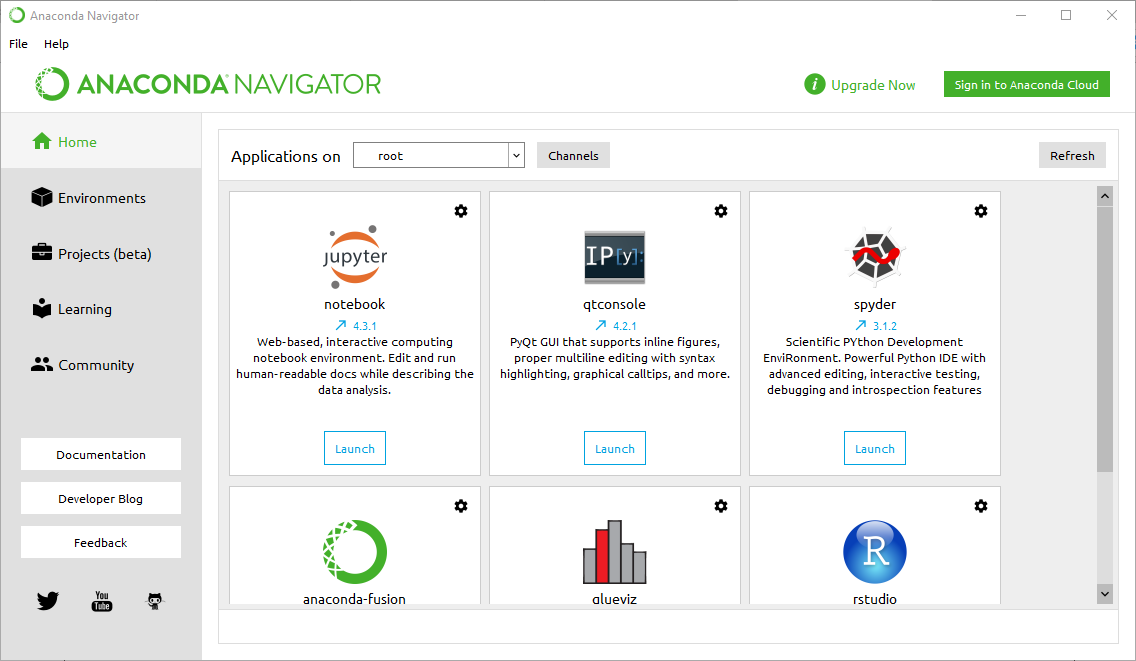
\includegraphics[width=0.7\linewidth]{imgs/AnacondaNavigator.png}}
  \caption{
  Interface graphique du navigateur Anaconda sur Windows
  }
\end{figure}
%\clearpage % flush figures 


% !split
\begin{block}{Notice}
Anaconda installe plusieurs exécutables pour développer en Python dans le répertoire \emph{anaconda/bin}, sans toujours créer des raccourcis sur le bureau ou dans un menu. Nous nous occuperons au tout début de la formation de créer des raccourcis pour pouvoir lancer l'application web \emph{Jupyter notebook}. Vous pouvez lancer le notebook depuis le navigateur Anaconda.
\end{block}

% !split
\section{Introduction: "Hello World!"}
C'est devenu une tradition que lorsque vous apprenez un nouveau langage de programmation, vous démarrez avec un programme permettant à l'ordinateur d'imprimer le message \emph{"Hello World!"}.

\bipy
In [1]: print("Hello World!")
Hello World!
\eipy

Félicitation! tout à l'heure vous avez fait votre ordinateur saluer le monde en anglais! La fonction \texttt{print()} est utilisée pour imprimer l’instruction entre les parenthèses. De plus, l'utilisation de guillemets simples \Verb?print('Hello World!')? affichera le même résultat. Le délimiteur de début et de fin doit être le même.

\bipy
In [2]: print('Hello World!')
Hello World!
\eipy

% !split
\section{Commentaires}

Au fur et à mesure que vos programmes deviennent plus grands et plus compliqués, ils deviennent plus difficiles à lire et à regarder un morceau de code et à comprendre ce qu'il fait ou pourquoi. Pour cette raison, il est conseillé d’ajouter des notes à vos programmes pour expliquer en langage naturel ce qu’il fait. Ces notes s'appellent des commentaires et commencent par le symbole \Verb!#!.

Voyez ce qui se passe lorsque nous ajoutons un commentaire au code précédent:

\bipy
In [3]: print('Hello World!') # Ceci est mon premier commentaire
Hello World!
\eipy
Rien ne change dans la sortie? Oui, et c’est très normal, l’interprète Python ignore cette ligne et ne renvoie rien. La raison en est que les commentaires sont écrits pour les humains, pour comprendre leurs codes, et non pour les machines.

% !split
\section{Nombres}

L'interpréteur Python agit comme une simple calculatrice: vous pouvez y taper une expression et l'interpréteur restituera la valeur. La syntaxe d'expression est simple: les opérateurs +, -, * et / fonctionnent comme dans la plupart des autres langages (par exemple, Pascal ou C); les parenthèses (\texttt{()}) peuvent être utilisées pour le regroupement. Par exemple:

\bipy
In [4]: 5+3
Out[4]: 8
In [5]: 2 - 9      # les espaces sont optionnels
Out[5]: -7
In [6]: 7 + 3 * 4  #la hiérarchie des opérations mathématique
Out[6]: 19
In [7]: (7 + 3) * 4  # est-elle respectées?
Out[7]: 40
# en python3 la division retourne toujours un nombre en virgule flottante
In [8]: 20 / 3
Out[8]: 6.666666666666667
In [9]: 7 // 2      # une division entière
Out[9]: 3
\eipy

% !split
On peut noter l’existence de l’opérateur \Verb!%! (appelé opérateur modulo). Cet opérateur fournit le reste de la division entière d’un nombre par un autre. Par exemple :

\bipy
In [10]: 7 % 2       # donne le reste de la division
Out[10]: 1
In [11]: 6 % 2
Out[11]: 0
\eipy

Les exposants peuvent être calculés à l'aide de doubles astérisques \texttt{**}.

\bipy
In [12]: 3**2
Out[12]: 9
\eipy

Les puissances de dix peuvent être calculées comme suit:

\bipy
In [13]: 3 * 2e3   # vaut 3 * 2000
Out[13]: 6000.0
\eipy
% !split
\section{Affectations (ou assignation)}

\subsection{variables}
Dans presque tous les programmes Python que vous allez écrire, vous aurez des variables. Les variables agissent comme des espaces réservés pour les données. Ils peuvent aider à court terme, ainsi qu’à la logique, les variables pouvant changer, d’où leur nom. C’est beaucoup plus facile en Python car aucune déclaration de variables n’est requise. Les noms de variable (ou tout autre objet Python tel que fonction, classe, module, etc.) commencent par une lettre majuscule ou minuscule (A-Z ou a-z). Ils sont sensibles à la casse (\texttt{VAR1} et \texttt{var1} sont deux variables distinctes). Depuis Python, vous pouvez utiliser n’importe quel caractère Unicode, il est préférable d’ignorer les caractères ASCII (donc pas de caractères accentués).

Si une variable est nécessaire, pensez à un nom et commencez à l'utiliser comme une variable, comme dans l'exemple ci-dessous:

% !split
Pour calculer l'aire d'un rectangle par exemple: \texttt{largeur} x \texttt{hauteur}:

\bipy
In [15]: largeur = 25
In [16]: hauteur = 40
In [17]: largeur    # essayer d'accéder à la valeur de la variable largeur
Out[17]: 25
\eipy

on peut également utiliser la fonction \texttt{print()} pour afficher la valeur de la variable \texttt{largeur}

\bipy
In [16]: print(largeur)
25
\eipy
Le produit de ces deux variables donne l'aire du rectangle:
\bipy
In [17]: largeur * hauteur  # donne l'aire du rectangle
Out[17]: 1000
\eipy
% !split
\begin{block}{Notice}
Notez ici que le signe égal (\texttt{=}) dans l'affectation ne doit pas être considéré comme \textbf{"est égal à"}. Il doit être \textbf{"lu"} ou interprété comme \textbf{"est définie par"}, ce qui signifie dans notre exemple:

\begin{quote}
La variable \texttt{largeur} est définie par la valeur 25 et la variable \texttt{hauteur} est définie par la valeur 40.
\end{quote}

\end{block}

\begin{block}{Warning}
Si une variable n'est pas \emph{définie} (assignée à une valeur), son utilisation vous donnera une erreur:

\bipy
In [18]: aire     # essayer d'accéder à une variable non définie
-----------------------------------------------------------------------
NameError                            Traceback (most recent call last)
<ipython-input-18-1b03529c1ce5> in <module>()
----> 1 aire     # essayer d'accéder à une variable non définie

NameError: name 'aire' is not defined
\eipy
\end{block}
% !split

Laissez-nous résoudre ce problème informatique (ou \textbf{bug} tout simplement)!. En d'autres termes, assignons la variable \texttt{aire} à sa valeur.

\bipy
In [19]: aire = largeur * hauteur
In [20]: aire  # et voila!
Out[20]: 1000
\eipy

\subsection{Noms de variables réservés (keywords)}
Certains noms de variables ne sont pas disponibles, ils sont réservés à python lui-même. Les mots-clés suivants (que vous pouvez afficher dans l'interpréteur avec la commande \texttt{help("keywords")}) sont réservés et ne peuvent pas être utilisés pour définir vos propres identifiants (variables, noms de fonctions, classes, etc.).

% !split
\bipy
In [20]: help("keywords")

Here is a list of the Python keywords.  Enter any keyword to get more help.

False               def                 if                  raise
None                del                 import              return
True                elif                in                  try
and                 else                is                  while
as                  except              lambda              with
assert              finally             nonlocal            yield
break               for                 not
class               from                or
continue            global              pass

# par exemple pour éviter d'écraser le nom réservé lambda
In [22]: Lambda = 630e-9
In [23]: Lambda
Out[23]: 6.3e-07
\eipy

% !split
\subsection{Les types}
Les types utilisés dans Python sont: integers, long integers, floats (double prec.), complexes, strings, booleans. La fonction \texttt{type()} donne le type de son argument
\paragraph{Le type int (integer : nombres entiers).}
Pour affecter (on peut dire aussi assigner) la valeur 20 à la variable nommée \texttt{age} :

\bipy
age = 20
\eipy
La fonction \texttt{print()} affiche la valeur de la variable :

\bipy
In [24]: print(age)
20
\eipy
La fonction \texttt{type()} retourne le type de la variable :
\bipy
type(age)
Out[25]: int
\eipy

% !split
\paragraph{Le type float (nombres en virgule flottante).}
\bipy
b = 17.0  # le séparateur décimal est un point (et non une virgule)
b
Out[26]: 17.0
In [27]: type(b)
Out[27]: float
In [28]: c = 14.0/3.0
    ...: c
Out[28]: 4.666666666666667
\eipy
Notation scientifique :
\bipy
In [29]: a = -1.784892e4
    ...: a
Out[29]: -17848.92
\eipy
% !split
\paragraph{Les fonctions mathématiques.}
Pour utiliser les fonctions mathématiques, il faut commencer par importer le module \texttt{math} :

\bipy
import math
\eipy
La fonction \texttt{help()} retourne la liste des fonctions et données d'un module.

Soit par exemple: \texttt{help('math')}

% !split

Pour appeler une fonction d'un module, la syntaxe est la suivante : \texttt{module.fonction(arguments)}

Pour accéder à une donnée d'un module : \texttt{module.data}

\bipy
 # donnée pi du module math (nombre pi)
In [32]: math.pi
Out[32]: 3.141592653589793
# fonction sin() du module math (sinus)
In [33]: math.sin(math.pi/4.0)
Out[33]: 0.7071067811865475
# fonction sqrt() du module math (racine carrée)
In [34]: math.sqrt(2.0)
Out[34]: 1.4142135623730951
# fonction exp() du module math (exponentielle)
In [35]: math.exp(-3.0)
Out[35]: 0.049787068367863944
# fonction log() du module math (logarithme népérien)
In [36]: math.log(math.e)
Out[36]: 1.0
\eipy

% !split
\paragraph{Le type complexe.}
Python possède par défaut un type pour manipuler les nombres complexes. La partie imaginaire est indiquée grâce à la lettre « \texttt{j} » ou « \texttt{J} ». La lettre mathématique utilisée habituellement, le « \texttt{i} », n’est pas utilisée en Python car la variable i est souvent utilisée dans les boucles.

\bipy
In [37]: a = 2 + 3j
    ...: type(a)
Out[37]: complex
In [38]: a
Out[38]: (2+3j)
\eipy
% !split
\begin{block}{Warning}
\bipy
In [39]: b = 1 + j
--------------------------------------------------------------
NameError                      Traceback (most recent call last)
<ipython-input-39-0f22d953f29e> in <module>()
----> 1 b = 1 + j

NameError: name 'j' is not defined
\eipy
Dans ce cas, on doit écrire la variable \texttt{b} comme suit:
\bipy
In [41]: b = 1 + 1j
    ...: b
Out[41]: (1+1j)
\eipy
sinon Python va considérer \texttt{j} comme variable non définie.
\end{block}

% !split
\paragraph{Le type str (string : chaîne de caractères).}
\bipy

In [43]: nom = 'Tounsi' # entre apostrophes
    ...: nom
Out[43]: 'Tounsi'
In [44]: type(nom)
Out[44]: str
In [45]: prenom = "Ali"  # on peut aussi utiliser les guillemets
    ...: prenom
Out[45]: 'Ali'
In [46]: print(nom, prenom)  # ne pas oublier la virgule
Tounsi Ali
\eipy
% !split
La concaténation désigne la mise bout à bout de plusieurs chaînes de caractères.
La concaténation utilise l'opérateur \texttt{+}:
\bipy
In [47]: chaine = nom + prenom  # concaténation de deux chaînes de caractères
    ...: chaine
Out[47]: 'TounsiAli'
\eipy
Vous voyez dans cet exemple que le nom et le prénom sont collé. Pour ajouter une espace entre ces deux chaînes de caractères:
\bipy
In [48]: chaine = prenom + ' ' + nom
    ...: chaine # et voila
Out[48]: 'Ali Tounsi'
\eipy

% !split
On peut modifier/ajouter une nouvelle chaîne à notre variable \texttt{chaine} par:
\bipy
In [49]: chaine = chaine + ' 22 ans'  # en plus court : chaine += ' 22 ans'
    ...: chaine
Out[49]: 'Ali Tounsi 22 ans'
\eipy

La fonction \texttt{len()} renvoie la longueur (\emph{length}) de la chaîne de caractères :

\bipy
In [53]: print(nom)
    ...: len(nom)
Tounsi
Out[53]: 6
\eipy
% !split
\paragraph{Indexage et slicing :}

\bccq
 +---+---+---+---+---+---+
|------------------------|
 | T | o | u | n | s | i |
 +---+---+---+---+---+---+
 |------------------------|
 0   1   2   3   4   5   6
 --->
-6  -5  -4  -3  -2  -1
                   <----
\eccq
\bipy
In [55]: nom[0]  # premier caractère (indice 0)
Out[55]: 'T'

In [56]: nom[:] # toute la chaine
Out[56]: 'Tounsi'

In [57]: nom[1] # deuxième caractère (indice 1)
Out[57]: 'o'
\eipy
% !split
\bipy
In [58]: nom[1:4]   # slicing
Out[58]: 'oun'

In [59]: nom[2:]  # slicing
Out[59]: 'unsi'

In [60]: nom[-1]   # dernier caractère (indice -1)
Out[60]: 'i'

In [61]: nom[-3:]    # slicing
Out[61]: 'nsi'

\eipy
% !split
\begin{block}{Warning}

On ne peut pas mélanger le type \texttt{str} et type \texttt{int}.

Soit par exemple:
\bipy
In [63]: chaine = '22'
    ...: annee_naissance = 2018 - chaine
----------------------------------------------------------
TypeError                  Traceback (most recent call last)
<ipython-input-63-8607078f78d2> in <module>()
      1 chaine = '22'
----> 2 annee_naissance = 2018 - chaine

TypeError: unsupported operand type(s) for -: 'int' and 'str'
\eipy
\end{block}
% !split
Pour corriger cette erreur, la fonction \texttt{int()} permet de convertir un type \texttt{str} en type \texttt{int}:

\bipy

In [64]: nombre = int(chaine)
In [65]: type(nombre) # et voila!
Out[65]: int
\eipy

Maintenant on peut trouver \Verb!annee_naissance! sans aucun problème:
\bipy
In [65]: annee_naissance = 2018 - nombre
    ...: annee_naissance
Out[65]: 1996
\eipy
% !split
\paragraph{ Formatage des chaînes}

Un problème qui se retrouve souvent, c’est le besoin d’afficher un message qui contient des valeurs de variables.

Soit le message: Bonjour Mr/Mme \texttt{prenom}, votre age est \texttt{age}.

La solution est d'utiliser la méthode \texttt{format()} de l'objet chaîne \texttt{str()} et le \Verb!{}! pour définir la valeur à afficher.

\bipy
print(" Bonjour Mr/Mme {}, votre age est {}.".format(prenom, age))
\eipy

% !split
\paragraph{Le type list (liste)}

Une liste est une structure de données.

Le premier élément d'une liste possède l'indice (l'index) 0.

Dans une liste, on peut avoir des éléments de plusieurs types.

\bipy
In [1]: info = ['Tunisie', 'Afrique', 3000, 36.8, 10.08]

In [2]: type(info)
Out[2]: list
\eipy
La liste info contient 5 éléments de types str, str, int, float et float

\bipy
In [3]: info
Out[3]: ['Tunisie', 'Afrique', 3000, 36.8, 10.08]

In [4]: print('Pays : ', info[0])    # premier élément (indice 0)
Pays :  Tunisie

In [5]: print('Age : ', info[2])     # le troisième élément a l'indice 2
Age :  3000

In [6]: print('Latitude : ', info[3]) # le quatrième élément a l'indice 3
Latitude :  36.8
\eipy

% !split
La fonction \texttt{range()} crée une liste d'entiers régulièrement espacés :

\bipy
In [7]: maliste = range(10) # équivalent à range(0,10,1)
   ...: type(maliste)
Out[7]: range
\eipy
Pour convertir une range en une liste, on applique la fonction \texttt{list()} à notre variable:
\bipy
In [8]: list(maliste)   # pour convertir range en une liste
Out[8]: [0, 1, 2, 3, 4, 5, 6, 7, 8, 9]
\eipy
On peut spécifier le début, la fin et l'intervalle d'une range:
\bipy
In [9]: maliste = range(1,10,2)   # range(début,fin non comprise,intervalle)
   ...: list(maliste)
Out[9]: [1, 3, 5, 7, 9]

In [10]: maliste[2] # le troisième élément a l'indice 2
Out[10]: 5
\eipy
% !split
On peut créer une liste de listes, qui s'apparente à un tableau à 2 dimensions (ligne, colonne) :

\bccq
0   1   2
10  11  12
20  21  22
\eccq

\bipy
In [11]: maliste = [[0, 1, 2], [10, 11, 12], [20, 21, 22]]
    ...: maliste[0]
Out[11]: [0, 1, 2]

In [12]: maliste[0][0]
Out[12]: 0

In [13]: maliste[2][1] # élément à la troisième ligne et deuxième colonne
Out[13]: 21

In [14]: maliste[2][1] = 78   # nouvelle affectation

In [15]: maliste
Out[15]: [[0, 1, 2], [10, 11, 12], [20, 78, 22]]
\eipy
% !split
\paragraph{Le type bool (booléen).}
Deux valeurs sont possibles : \texttt{True} et \texttt{False}

\bipy
In [16]: choix = True # NOTE: "True" différent de "true"
    ...: type(choix)
Out[16]: bool
\eipy

% !split
Les opérateurs de comparaison :




\begin{quote}
\begin{tabular}{lll}
\hline
\multicolumn{1}{c}{ Opérateur } & \multicolumn{1}{c}{ Signification } & \multicolumn{1}{c}{ Remarques } \\
\hline
\texttt{<}  & strictement inférieur &                                   \\
\texttt{<=} & inférieur ou égal     &                                   \\
\texttt{>}  & strictement supérieur &                                   \\
\texttt{>=} & supérieur ou égal     &                                   \\
\texttt{==} & égal                  & Attention : deux signes \texttt{==} \\
\Verb?!=? & différent             &                                   \\
\hline
\end{tabular}
\end{quote}

\noindent
\bipy
In [17]: b = 10
    ...: b > 8
Out[17]: True

In [18]: b == 5
Out[18]: False

In [19]: b != 5
Out[19]: True

In [20]: 0 <= b <= 20
Out[20]: True
\eipy
% !split
Les opérateurs logiques : \texttt{and}, \texttt{or}, \texttt{not}

\bipy
In [21]: note = 13.0

In [22]: mention_ab = note >= 12.0 and note < 14.0

In [23]: # ou bien : mention_ab = 12.0 <= note < 14.0

In [24]: mention_ab
Out[24]: True
\eipy

\bipy
In [25]: not mention_ab
Out[25]: False

In [26]: note == 20.0 or note == 0.0
Out[26]: False
\eipy
% !split
L'opérateur \texttt{in} s'utilise avec des chaînes (type \texttt{str}) ou des listes (type \texttt{list}).

Pour une chaînes:
\bipy
In [30]: chaine = 'Bonsoir'
    ...: #la sous-chaîne 'soir' fait-elle partie de la chaîne 'Bonsoir' ?

In [31]: resultat = 'soir' in chaine
    ...: resultat
Out[31]: True
\eipy
% !split
Pour une liste:

\bipy

In [32]: maliste = [4, 8, 15]
    ...: #le nombre entier 9 est-il dans la liste ?

In [33]: 9 in maliste
Out[33]: False

In [34]: 8 in maliste
Out[34]: True

In [35]: 14 not in maliste
Out[35]: True
\eipy

% !split
\section{Les conditions}
\subsection{L'instruction \texttt{if} }
En programmation, nous avons toujours besoin de la notion de condition pour permettre à un programme de s'adapter à différents cas de figure.

\begin{block}{Syntaxe }

\bpycod
if expression: # ne pas oublier le signe de ponctuation ':'
    "bloc d'instructions" # attention à l'indentation (1 Tab ou 4 * Espaces)
# suite du programme
\epycod
\begin{itemize}
\item Si l'expression est vraie (\texttt{True}) alors le bloc d'instructions est exécuté.

\item Si l'expression est fausse (\texttt{False}) on passe directement à la suite du programme.
\end{itemize}

\noindent
\end{block}


% !split
\paragraph{Exemple 1: Note sur 20.}
Dans cet exemple nous allons tester si la note entrée par l'utilisateur. Si la note est > 10 on doit recevoir le message: "J'ai la moyenne" sinon il va rien faire.
\bpycod
chaine = input("Note sur 20 : ")
note = float(chaine)
if note >= 10.0:
    # ce bloc est exécuté si l'expression (note >= 10.0) est vraie
    print("J'ai la moyenne")

# suite du programme
print("Fin du programme")
\epycod

\begin{block}{Notice}
\begin{itemize}
\item Les blocs de code sont délimités par l'indentation.

\item L'indentation est obligatoire dans les scripts.
\end{itemize}

\noindent
\end{block}

% !split
\subsection{L'instruction \texttt{else} }

Une instruction \texttt{else} est toujours associée à une instruction \texttt{if}.

\begin{block}{Syntaxe }

\bpycod
if expression:
    "bloc d'instructions 1"    # attention à l'indentation (1 Tab ou 4 * Espaces)
else:                          # else est au même niveau que if
    "bloc d'instructions 2"    # attention à l'indentation
# suite du programme
\epycod
\begin{itemize}
\item Si l'expression est vraie (\texttt{True}) alors le bloc d'instructions 1 est exécuté.

\item Si l'expression est fausse (\texttt{False}) alors c'est le bloc d'instructions 2 qui est exécuté.
\end{itemize}

\noindent
\end{block}


% !split
\paragraph{Exemple 2 : moyenne.}
Dans cet exemple nous allons tester si la note entrée par l'utilisateur. Si la note est > 10 on doit recevoir le message: "J'ai la moyenne" sinon il va afficher "C'est en dessous de la moyenne".

\bpycod
chaine = input("Note sur 20 : ")
note = float(chaine)
if note >= 10.0:
    # ce bloc est exécuté si l'expression (note >= 10.0) est vraie
    print("J'ai la moyenne")
else:
    # ce bloc est exécuté si l'expression (note >= 10.0) est fausse
    print("C'est en dessous de la moyenne")
print("Fin du programme")
\epycod
% !split
Ou bien encore:
\bpycod
chaine = input("Note sur 20 : ")
note = float(chaine)
if note > 20.0 or note < 0.0:
    print("Note invalide !")
else:
    if note >= 10.0:
        print("J'ai la moyenne")
        if note == 20.0:
            # ce bloc est exécuté si l'expression (note == 20.0) est vraie
            print("C'est même excellent !")
    else:
        print("C'est en dessous de la moyenne")
        if note == 0.0:
            # ce bloc est exécuté si l'expression (note == 0.0) est vraie
            print("... lamentable !")
print("Fin du programme")
\epycod

% !split
\subsection{L'instruction \texttt{elif} }
\begin{block}{Syntaxe }

\bpycod
if expression 1:
    "bloc d'instructions 1"
elif expression 2:
    "bloc d'instructions 2"
elif expression 3:
    "bloc d'instructions 3"    # ici deux instructions elif, mais il n'y a pas de limitation
else:
    "bloc d'instructions 4"
# suite du programme
\epycod
\begin{itemize}
\item Si l'expression 1 est vraie alors le bloc d'instructions 1 est exécuté, et on passe à la suite du programme.

\item Si l'expression 1 est fausse alors on teste l'expression 2 :

\item si l'expression 2 est vraie on exécute le bloc d'instructions 2, et on passe à la suite du programme.

\item si l'expression 2 est fausse alors on teste l'expression 3, etc.
\end{itemize}

\noindent
\end{block}
% !split
Le bloc d'instructions 4 est donc exécuté si toutes les expressions sont fausses (c'est le bloc "par défaut").

Parfois il n'y a rien à faire. Dans ce cas, on peut omettre l'instruction \texttt{else} :

\bpycod
if expression 1:
    "bloc d'instructions 1"
elif expression 2:
    "bloc d'instructions 2"
elif expression 3:
    "bloc d'instructions 3"
# suite du programme
\epycod
% !split
L'instruction \texttt{elif} évite souvent l'utilisation de conditions imbriquées (et souvent compliquées).

\paragraph{Exemple 3 : moyenne-bis.}
On peut tester plusieurs possibilités avec une syntaxe beaucoup plus propre avec les instructions \texttt{if-elif-else}:
\bpycod
note = float(input("Note sur 20 : "))
if note == 0.0:
    print("C'est en dessous de la moyenne")
    print("... lamentable!")
elif note == 20.0:
    print("J'ai la moyenne")
    print("C'est même excellent !")
elif 0 < note < 10:    # ou bien : elif 0.0 < note < 10.0:
    print("C'est en dessous de la moyenne")
elif note >= 10.0 and note < 20.0:   # ou bien : elif 10.0 <= note < 20.0:
    print("J'ai la moyenne")
else:
    print("Note invalide !")
print("Fin du programme")
\epycod
% !split
\section{Les boucles}
\subsection{L'instruction \texttt{while} }

\begin{block}{Syntaxe }

\bpycod
while expression:           # ne pas oublier le signe de ponctuation ':'
    "bloc d'instructions"   # attention à l'indentation (1 Tab ou 4 * Espaces)
# suite du programme
\epycod
\begin{itemize}
\item Si l'expression est vraie (\texttt{True}) le bloc d'instructions est exécuté, puis l'expression est à nouveau évaluée.

\item Le cycle continue jusqu'à ce que l'expression soit fausse (\texttt{False}) : on passe alors à la suite du programme.
\end{itemize}

\noindent
\end{block}
% !split
\paragraph{Exemple 1 : un script qui compte de 1 à 4.}
\bpycod
# initialisation de la variable de comptage
compteur = 0
while compteur < 5:
    # ce bloc est exécuté tant que la condition (compteur < 5) est vraie
    print(compteur)
    compteur +=  1    # incrémentation du compteur,  compteur = compteur + 1
print(compteur)
print("Fin de la boucle")
\epycod
% !split
\paragraph{Exemple 2 : Table de multiplication par 8.}
\bpycod
compteur = 1         # initialisation de la variable de comptage
while compteur <= 10:
    # ce bloc est exécuté tant que la condition (compteur <= 10) est vraie
    print(compteur, '* 8 =', compteur*8)
    compteur += 1    # incrémentation du compteur, compteur = compteur + 1
print("Et voilà !")
\epycod
% !split
\paragraph{Exemple 3 : Affichage de l'heure courante.}
\bpycod
import time     # importation du module time
quitter = 'n'   # initialisation
while quitter != 'o':
    # ce bloc est exécuté tant que la condition est vraie
    # strftime() est une fonction du module time
    print('Heure courante ', time.strftime('%H:%M:%S'))
    quitter = input("Voulez-vous quitter le programme (o/n) ? ")
print("A bientôt")
\epycod
% !split
\subsection{L'instruction \texttt{for} }

\begin{block}{Syntaxe }

\bpycod
for élément in séquence :     # ne pas oublier le signe de ponctuation ':'
    "bloc d'instructions"     # attention à l'indentation (1 Tab ou 4 * Espaces)
# suite du programme
\epycod
\end{block}

Les éléments de la séquence sont issus d'une chaîne de caractères ou bien d'une liste.
% !split
\paragraph{Exemple 1 : séquence de caractères.}
\bpycod
chaine = 'Bonsoir'
for lettre in chaine:  # lettre est la variable d'itération
    print(lettre)
print("Fin de la boucle")
\epycod

La variable lettre est initialisée avec le premier élément de la séquence ('B').
Le bloc d'instructions est alors exécuté.

Puis la variable lettre est mise à jour avec le second élément de la séquence ('o') et le bloc d'instructions à nouveau exécuté...

Le bloc d'instructions est exécuté une dernière fois lorsqu'on arrive au dernier élément de la séquence ('r').
% !split
\paragraph{Fonction \texttt{range()}.}
L'association avec la fonction \texttt{range()} est très utile pour créer des séquences automatiques de nombres entiers :

\bpycod
for i in range(1, 5):
    print(i)
print("Fin de la boucle")
\epycod
% !split
\paragraph{Exemple 2 : Table de multiplication.}
La création d'une table de multiplication paraît plus simple avec une boucle \texttt{for} qu'avec une boucle \texttt{while} :

\bpycod
for compteur in range(1,11):
    print(compteur, '* 8 =', compteur*8)
print("Et voilà !")
\epycod
% !split
\paragraph{Exemple 3 : calcul d'une somme.}
Soit, par exemple, l'expression de la somme suivante:
\[
s = \sum_{i = 0}^{100} \sqrt{\frac{i \pi}{100}} sin(\frac{i \pi}{100})
\]

\bpycod
from math import sqrt, sin, pi
s = 0.0 # # intialisation de s
for i in range(101):
    s+= sqrt(i * pi/100) * sin(i * pi/100)   # équivalent à s = s + sqrt(x) * sin(x)
# Affichage de la somme
print(s)
\epycod
% !split
\subsection{L'instruction break}

L'instruction break provoque une sortie immédiate d'une boucle \texttt{while} ou d'une boucle \texttt{for}.

Dans l'exemple suivant, l'expression \texttt{True} est toujours ... vraie : on a une boucle sans fin.

L'instruction \texttt{break} est donc le seul moyen de sortir de la boucle.
% !split
\paragraph{Exemple : Affichage de l'heure courante.}
\bpycod
import time     # importation du module time
while True:
    # strftime() est une fonction du module time
    print('Heure courante ', time.strftime('%H:%M:%S'))
    quitter = input('Voulez-vous quitter le programme (o/n) ? ')
    if quitter == 'o':
        break
print("A bientôt")
\epycod

\begin{block}{Notice}
Si vous connaissez le nombre de boucles à effectuer, utiliser une boucle \texttt{for}.
Autrement, utiliser une boucle \texttt{while} (notamment pour faire des boucles sans fin).
\end{block}
% !split
\section{Les fonctions}

Nous avons déjà vu beaucoup de fonctions : \texttt{print()}, \texttt{type()}, \texttt{len()}, \texttt{input()}, \texttt{range()}...

Ce sont des fonctions pré-définies (\href{{https://docs.python.org/fr/3/library/functions.html}}{Fonctions natives}).

Nous avons aussi la possibilité de créer nos propres fonctions!

% !split
\subsection{Intérêt des fonctions}

Une fonction est une portion de code que l'on peut appeler au besoin (c'est une sorte de sous-programme).

L'utilisation des fonctions évite des redondances dans le code : on obtient ainsi des programmes plus courts et plus lisibles.

Par exemple, nous avons besoin de convertir à plusieurs reprises des degrés Celsius en degrés Fahrenheit :
$$T_F = T_C \times 1,8 + 32 $$

\bpycod
print(100 * 1.8 + 32.0)
\epycod

\bpycod
print(37.0 * 1.8 + 32.0)
\epycod

\bpycod
print(233.0 * 1.8 + 32.0)
\epycod
% !split
La même chose en utilisant une fonction :

\bpycod
def fahrenheit(degre_celsius):
        """
        Conversion degré Celsius en degré Fahrenheit
        """
        print(degre_celsius * 1.8 + 32.0)
\epycod

\bpycod
fahrenheit(100)
\epycod

\bpycod
fahrenheit(37)
\epycod

\bpycod
temperature = 220
fahrenheit(temperature)
\epycod
% !split
\subsection{L'instruction def}

\begin{block}{Syntaxe }

\bpycod
def nom_de_la_fonction(parametre1, parametre2, parametre3, ...):
    """
    Documentation
    qu'on peut écrire
    sur plusieurs lignes
    """     # docstring entouré de 3 guillemets (ou apostrophes)

    "bloc d'instructions"     # attention à l'indentation

    return resultat            # la fonction retourne le contenu de la variable resultat
\epycod
\end{block}
% !split
\paragraph{Exemple : ma première fonction.}
\bpycod
def mapremierefonction():         # cette fonction n'a pas de paramètre
    """
    Cette fonction affiche 'Bonjour'
    """
    print("Bonjour")
    return                         # cette fonction ne retourne rien ('None')
    # l'instruction return est ici facultative
\epycod

\bpycod
mapremierefonction()
\epycod

\bpycod
help(mapremierefonction)
\epycod

% ------------------- end of main content ---------------

% #ifdef PREAMBLE
\end{document}
% #endif

